\section{Massima verosimiglianza}\label{sec:mle}

\subsection{Stimatori}\label{sec:stimatori}

\begin{definizione}{Campione casuale}{campione}
Un \emph{campione casuale} è una collezione di variabili aleatorie i.i.d.:
\[
X_1, X_2, \dots, X_n
\]
Le realizzazioni osservate sono i dati: \( x_1, x_2, \dots, x_n \).
\end{definizione}

Ad esempio, possiamo raccogliere le altezze o le pressioni sanguigne di un gruppo di individui (\Cref{ex:pressione}). Questi dati rappresentano realizzazioni di variabili aleatorie, che modellano fenomeni osservabili in un contesto sperimentale o reale.
\begin{esempio}{Pressione sanguigna}{pressione}
Raccolgo le seguenti misurazioni di pressione da un gruppo di studenti:
\[
115, \quad 135, \quad 127, \quad 148, \quad 126
\]
Posso ipotizzare che:
\[
X_1, X_2, \dots, X_n \sim \mathcal{N}(\mu, \sigma^2)
\quad \Rightarrow \quad \mu < 200 \text{ con alta probabilità}
\]
\end{esempio}

\begin{definizione}{Statistica inferenziale}{inferenziale}
Lo scopo della statistica inferenziale è quello di trarre conclusioni sulla \emph{legge delle \( X_i \)} a partire dai dati osservati \( x_1, \dots, x_n \).
\end{definizione}

Per realizzare questo obiettivo, utilizziamo funzioni dei dati osservati che riassumono l'informazione rilevante contenuta nel campione. Queste funzioni sono chiamate \textbf{statistiche}.

\begin{definizione}{Statistica}{statistica}
Una \textbf{statistica} è una variabile aleatoria che è funzione deterministica del campione, ovvero:
\[
T = f(X_1, X_2, \dots, X_n)
\]
\end{definizione}

In particolare, quando una statistica viene usata per fornire una stima di un parametro incognito del modello (ad esempio, la media o la varianza della popolazione), essa prende il nome di \textbf{stimatore}.

Informalmente, uno \textbf{stimatore} di un parametro \( \theta \) è una statistica \( \hat{\theta} = f(X_1, \dots, X_n) \) la cui legge è in qualche modo concentrata attorno a \( \theta \).

\begin{definizione}{Stimatore}{stimatore}
Uno \textbf{stimatore} è una funzione dei dati che serve a stimare un parametro ignoto (es. la media \( \mu \)) della distribuzione da cui proviene il campione.
\end{definizione}

Tra i più comuni stimatori, troviamo ad esempio:
\begin{itemize}
  \item La \textbf{media campionaria}:
  \[
  \bar{X} = \frac{1}{n} \sum_{i=1}^n X_i
  \]
  \item La \textbf{mediana campionaria}, ovvero \( X_{(n/2)} \)
\end{itemize}
Nel caso normale (gaussiano), media e mediana coincidono. In generale, no.

\begin{definizione}{Stimatore consistente}{consistenza}
Uno \textbf{stimatore consistente} di un parametro \( \theta \) è una famiglia di statistiche \( \hat{\theta}_n \), con \( n = 1, 2, \dots \), tale che:
\[
    \hat{\theta}_n \xrightarrow[P]{n \to \infty} \theta \quad \text{(convergenza in probabilità)}
\]
Cioè:
\[
\forall \varepsilon > 0, \quad P(|\hat{\theta}_n - \theta| > \varepsilon) \xrightarrow{n \to \infty} 0
\]
Operativamente, è sufficiente che:
\[
\mathbb{E}[\hat{\theta}_n] \xrightarrow{n \to \infty} \theta \quad \text{e} \quad \text{Var}(\hat{\theta}_n) \xrightarrow{n \to \infty} 0
\]
\end{definizione}

\begin{figure}[ht]
\centering
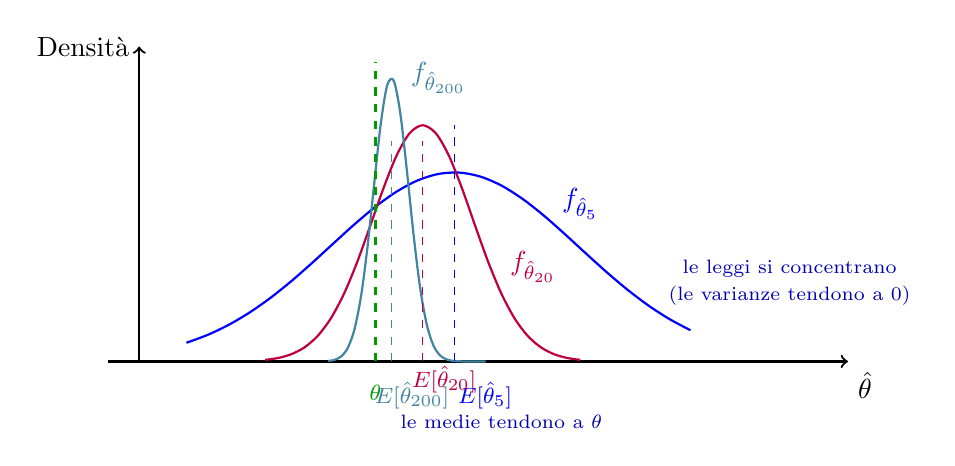
\begin{tikzpicture}[scale=2]

  % Assi
  \draw[->, thick] (-0.2, 0) -- (4.5, 0) node[below right] {$\hat{\theta}$};
  \draw[->, thick] (0, 0) -- (0, 2) node[left] {Densità};

  % Distribuzione larga - n piccolo
  \draw[domain=0.3:3.5, smooth, variable=\x, thick, blue]
    plot ({\x}, {1.2*exp(-0.8*(\x-2)^2)});
  \node[blue] at (2.8,1) {$f_{\hat{\theta}_5}$};

  % Distribuzione intermedia - n medio
  \draw[domain=0.8:2.8, smooth, variable=\x, thick, purple]
    plot ({\x}, {1.5*exp(-5*(\x-1.8)^2)});
  \node[purple] at (2.5,0.6) {$f_{\hat{\theta}_{20}}$};

  % Distribuzione stretta - n grande
  \draw[domain=1.2:2.2, smooth, variable=\x, thick, cyan!60!black]
    plot ({\x}, {1.8*exp(-40*(\x-1.6)^2)});
  \node[cyan!60!black] at (1.9,1.8) {$f_{\hat{\theta}_{200}}$};

  % Linea verticale per theta reale
  \draw[dashed, thick, green!60!black] (1.5, 0) -- (1.5, 1.9);
  \node[below=5pt, green!60!black] at (1.5, 0) {\footnotesize $\theta$};

  % Medie delle stime - con altezze alternate
  \draw[dashed, blue] (2, 0) -- (2, 1.5);
  \node[below left=4pt, blue] at (2.5, 0) {\footnotesize $\mathbb{E}[\hat{\theta}_5]$};

  \draw[dashed, purple] (1.8, 0) -- (1.8, 1.4);
  \node[below right=4pt, purple] at (1.6, 0.1) {\footnotesize $\mathbb{E}[\hat{\theta}_{20}]$};

  \draw[dashed, cyan!60!black] (1.6, 0) -- (1.6, 1.4);
  \node[below left=4pt, cyan!60!black] at (2.1, 0) {\footnotesize $\mathbb{E}[\hat{\theta}_{200}]$};

  % Annotazioni testuali
  \node[right] at (3.3, 0.5) {\scriptsize \textcolor{blue!70!black}{\shortstack{le leggi si concentrano\\(le varianze tendono a 0)} }};
  \node[below=16pt, align=center, text=blue!70!black] at (2.3, 0) {\scriptsize le medie tendono a $\theta$};
\end{tikzpicture}

\caption{Illustrazione della consistenza: la distribuzione di $\hat{\theta}_n$ si concentra attorno a $\theta$ all'aumentare di $n$.}
\label{fig:consistenza-stimatore}
\end{figure}

\begin{definizione}{Stimatore corretto}{correttezza}
Uno \textbf{stimatore corretto} di un parametro \( \theta \) è una statistica \( \hat{\theta} \) per cui:
\[
\mathbb{E}[\hat{\theta}] = \theta
\]
\end{definizione}

In caso contrario, lo stimatore è detto \textbf{distorto}, e la differenza
\[
\mathbb{E}[\hat{\theta}] - \theta
\]
è chiamata \textbf{bias} (errore sistematico).

\begin{nota}{Media campionaria}{}
Ricordiamo che:
\[
\bar{X} = \frac{1}{n} \sum_{i=1}^n X_i
\quad \Rightarrow \quad
\mathbb{E}[\bar{X}] = \mu, \quad
\mathrm{Var}(\bar{X}) = \frac{\sigma^2}{n}
\]

La media campionaria \( \bar{X} \) è \textbf{consistente e corretta}.
\end{nota}

\begin{nota}{Varianza campionaria}{varianza-campionaria}
La \textbf{varianza campionaria} è definita come:
\[
S_X^2 = \frac{1}{n - 1} \sum_{i=1}^n (X_i - \bar{X})^2
\]
La \textbf{deviazione standard campionaria} è:
\[
S_X = \sqrt{S_X^2} = \sqrt{\frac{1}{n - 1} \sum_{i=1}^n (X_i - \bar{X})^2}
\]
Entrambe le statistiche \( S_X^2 \) e \( S_X \) sono \textbf{consistenti} per \( \sigma^2 \) e \( \sigma \), rispettivamente. Tuttavia:
\[
\mathbb{E}[S_X^2] = \sigma^2 \quad \text{(corretto)}
\qquad \text{ma} \qquad
\mathbb{E}[S_X] < \sigma \quad \text{(distorto)}
\]
In particolare, se \(X_i \sim \mathcal{N}(\mu, \sigma^2)\) si dimostra che:
\[
\mathrm{Var}(S_X^2) = \frac{2\sigma^4}{n-1}
\quad \Rightarrow \quad
S_X^2 \text{ è consistente}
\]
mentre \( S_X \) è distorto perché:
\begin{align*}
    \mathbb{E}[{S_X}^2] = \sigma^2 ,\quad 0 < \text{Var}(S_X) = \mathbb{E}[{S_X}^2] - {\mathbb{E}[{S_X}]}^2 \quad &\Longrightarrow \quad {\mathbb{E}[S_X]}^2 < \sqrt{\mathbb{E}[{S_X}^2]} = \sigma^2 \\
    &\Longrightarrow \quad {\mathbb{E}[S_X]} < \sigma
\end{align*}
\end{nota}

Uno degli approcci più diffusi per stimare i parametri incogniti di un modello statistico è il metodo della \textbf{massima verosimiglianza}. L'idea di base è semplice: tra tutti i possibili valori del parametro, scegliamo quello che rende i dati osservati più "probabili".

\subsection{Definizione}

Se il modello prevede una densità (o massa) di probabilità parametrica \( f(x; \theta) \), e abbiamo a disposizione un campione di osservazioni \( x_1, \dots, x_n \), allora consideriamo la funzione di verosimiglianza come una funzione del parametro \( \theta \), e ne cerchiamo il massimo.

\begin{definizione}{Massima verosimiglianza}{mle}
Dato un campione i.i.d.\ \( X_1, \dots, X_n \sim f(x; \theta) \), la \textbf{funzione di verosimiglianza} è definita come:
\[
L(\theta; x_1, \dots, x_n) = \prod_{i=1}^n f(x_i; \theta)
\]
Lo \textbf{stimatore di massima verosimiglianza} (MLE) è il valore del parametro che massimizza la funzione di verosimiglianza:
\[
\hat{\theta}_{\text{MLE}} = \arg\max_{\theta} L(\theta; x_1, \dots, x_n)
\]
\end{definizione}

\begin{nota}{Il parametro \( \theta \)}{par-theta}
    Normalmente, il parametro \( \theta \) è un vettore \( \theta = (\theta_1,
    \theta_2, \ldots, \theta_k) \).
\end{nota}

In pratica, invece della funzione \( L \), si lavora spesso con la \emph{log-verosimiglianza}:
\[
\ell(\theta) = \log L(\theta; x_1, \dots, x_n) = \sum_{i=1}^n \log f(x_i; \theta)
\]
Poiché il logaritmo è strettamente crescente, il valore che massimizza \( \ell(\theta) \) è lo stesso che massimizza \( L(\theta) \), ma l’analisi è spesso più semplice con somme piuttosto che prodotti.

\begin{esempio}{MLE per la distribuzione Gamma}{mle-gamma}
Supponiamo che \( X_1, \dots, X_n \) siano variabili aleatorie indipendenti e distribuite secondo la legge \( \mathrm{Gamma}(\alpha, \beta) \), con densità:
\[
f(x; \alpha, \beta) = \frac{\beta^\alpha}{\Gamma(\alpha)} x^{\alpha - 1} e^{-\beta x}, \quad x > 0
\]

\textbf{1. Funzione di verosimiglianza.}  
Per un campione osservato \( x_1, \dots, x_n \), la funzione di verosimiglianza è:
\[
L(\alpha, \beta; x_1, \dots, x_n) = \prod_{i=1}^n \frac{\beta^\alpha}{\Gamma(\alpha)} x_i^{\alpha - 1} e^{-\beta x_i}
= \left(\frac{\beta^\alpha}{\Gamma(\alpha)}\right)^n \prod_{i=1}^n x_i^{\alpha - 1} e^{-\beta x_i}
\]

\textbf{2. Log-verosimiglianza.}  
Per semplificare il calcolo si prende il logaritmo:
\[
\ell(\alpha, \beta) = n\alpha \log \beta - n \log \Gamma(\alpha) + (\alpha - 1) \sum_{i=1}^n \log x_i - \beta \sum_{i=1}^n x_i
\]

\textbf{3. Massimizzazione.}  
Deriviamo rispetto a \( \beta \) e poniamo la derivata pari a zero:
\[
\frac{\partial \ell}{\partial \beta} = \frac{n\alpha}{\beta} - \sum_{i=1}^n x_i = 0 \quad \Rightarrow \quad
\hat{\beta} = \frac{n\alpha}{\sum x_i} = \frac{\alpha}{\bar{x}}
\]

Dove \( \bar{x} = \frac{1}{n} \sum x_i \) è la media campionaria.

\textbf{4. Derivata rispetto ad \( \alpha \).}  
Risulta più complicata, e coinvolge la funzione digamma \( \psi(\alpha) = \frac{d}{d\alpha} \log \Gamma(\alpha) \):
\[
\frac{\partial \ell}{\partial \alpha} = n \log \beta - n \psi(\alpha) + \sum \log x_i
\]
Questa equazione si risolve numericamente (es. metodo di Newton-Raphson) per ottenere \( \hat{\alpha} \).

\medskip
\textbf{Conclusione.} Gli stimatori MLE per \( \mathrm{Gamma}(\alpha, \beta) \) sono dati da:
\[
\hat{\beta} = \frac{\hat{\alpha}}{\bar{x}}, \quad \hat{\alpha} \text{ ottenuto risolvendo: } \log \hat{\beta} - \psi(\hat{\alpha}) + \frac{1}{n} \sum \log x_i = 0
\]
\end{esempio}


\subsection{Esempi notevoli}
\subsubsection{Distribuzione esponenziale}

Consideriamo un campione casuale \( X_1, \dots, X_n \sim \mathrm{expo}(\lambda) \), con densità:
\[
    f(x;\lambda) = \mathrm{expo}(\lambda) = \lambda e^{-\lambda x}, \quad x \geq 0
\]

\begin{esempio}{MLE per la legge esponenziale}{mle-exp}
La log-verosimiglianza associata al campione è:
\[
\ell(\lambda) = \sum_{i=1}^n \log f(x_i; \lambda) = \sum_{i=1}^n \left( \log \lambda - \lambda x_i \right)
= n \log \lambda - \lambda \sum_{i=1}^n x_i
\]

La funzione è concava, poiché la derivata seconda è negativa:
\[
\ell''(\lambda) = -\frac{n}{\lambda^2} < 0
\]

Derivando la log-verosimiglianza e ponendo uguale a zero otteniamo:
\[
\ell'(\lambda) = \frac{n}{\lambda} - \sum_{i=1}^n x_i = 0
\quad \Rightarrow \quad
\hat{\lambda} = \frac{n}{\sum x_i} = \left( \bar{x} \right)^{-1}
\]

\medskip
\textbf{Conclusione:} lo stimatore di massima verosimiglianza per \( \lambda \) è:
\[
T = \left( \bar{X} \right)^{-1}
\]

Questo esempio mostra che, nel caso esponenziale, la media campionaria \( \bar{X} \) è uno stimatore corretto della media teorica \( \frac{1}{\lambda} \). Poiché \( \bar{X} \) è corretta per la media, il suo inverso \( T \) è uno stimatore corretto per \( \lambda \) — e coincide con l’MLE.
\end{esempio}

\subsubsection{Legge uniforme}

Consideriamo un campione casuale \( X_1, \dots, X_n \sim \mathrm{unif}(0,a) \), con densità:
\[
    f(x;a) = \mathrm{unif}(0,a) = \frac{1}{a}
\]
\begin{esempio}{MLE per la legge uniforme}{mle-unif}

La funzione di verosimiglianza è:
\[
L(a) = \prod_{i=1}^n f(x_i; a) = 
\begin{cases}
\frac{1}{a^n} & \text{se } a \geq \max x_i \\
0 & \text{altrimenti}
\end{cases}
\]

La log-verosimiglianza è:
\[
\ell(a) = \log L(a) = 
\begin{cases}
- n \log a & \text{se } a \geq \max x_i \\
-\infty & \text{altrimenti}
\end{cases}
\]

Poiché \( \ell(a) \) decresce in \( a \), per massimizzarla bisogna scegliere il valore minimo ammissibile:
\[
\hat{a}_{\text{MLE}} = \max x_i
\]

\medskip
\textbf{Conclusione:} lo stimatore MLE per \( a \) è:
\[
Y := \max_{i=1,\dots,n} X_i
\]

\medskip

Questo stimatore è \emph{consistente} ma \emph{distorto}. Infatti:
\[
\mathbb{E}(Y) = \frac{n}{n+1} a
\quad \Rightarrow \quad
Y \text{ sottostima sistematicamente } a
\]

\medskip
\textbf{Correzione del bias:}
\[
Y_{\text{adj}} := \frac{n+1}{n} Y = \frac{n+1}{n} \max X_i
\]

Questo nuovo stimatore \( Y_{\text{adj}} \) è \textbf{corretto} e anch'esso consistente.

\begin{nota}{Bias degli MLE}{note:bias-mle}
Lo stimatore di massima verosimiglianza è spesso \emph{consistente} ma \emph{non corretto}. In molti casi, è possibile applicare una correzione (bias correction) per ottenere uno stimatore corretto mantenendo la consistenza.
\end{nota}
\end{esempio}


\subsubsection{Distribuzione normale}

Consideriamo il caso classico in cui \( X_1, \dots, X_n \sim \mathcal{N}(\mu, \sigma^2) \), con entrambi i parametri \( \mu \) e \( \sigma^2 \) ignoti.

\begin{esempio}{MLE per la legge normale}{mle-norm}
La densità della normale è:
\[
f(x; \mu, \sigma^2) = \frac{1}{\sqrt{2\pi \sigma^2}} \exp\left( -\frac{(x - \mu)^2}{2\sigma^2} \right)
\]

La log-verosimiglianza per un campione è:
\[
\ell(\mu, \sigma^2) = \sum_{i=1}^n \log f(x_i; \mu, \sigma^2) =
- \frac{n}{2} \log(2\pi) - \frac{n}{2} \log \sigma^2 - \frac{1}{2\sigma^2} \sum_{i=1}^n (x_i - \mu)^2
\]

\medskip
\textbf{Calcolo degli MLE:}
\begin{itemize}
  \item Derivando rispetto a \( \mu \) e ponendo uguale a zero:
  \[
  \frac{\partial \ell}{\partial \mu} = \frac{1}{\sigma^2} \sum_{i=1}^n (x_i - \mu) = 0
  \quad \Rightarrow \quad
  \hat{\mu} = \bar{x} = \frac{1}{n} \sum_{i=1}^n x_i
  \]

  \item Derivando rispetto a \( \sigma^2 \) e ponendo uguale a zero:
  \[
  \frac{\partial \ell}{\partial \sigma^2} = -\frac{n}{2\sigma^2} + \frac{1}{2\sigma^4} \sum_{i=1}^n (x_i - \bar{x})^2 = 0
  \quad \Rightarrow \quad
  \hat{\sigma}^2 = \frac{1}{n} \sum_{i=1}^n (x_i - \bar{x})^2
  \]
\end{itemize}

\medskip
\textbf{Conclusione:} gli stimatori di massima verosimiglianza sono:
\[
\hat{\mu} = \bar{X}, \qquad \hat{\sigma}^2 = \mathbb{S}^2 = \frac{1}{n} \sum_{i=1}^n (X_i - \bar{X})^2
\]

\medskip
\textbf{Osservazioni:}
\begin{itemize}
  \item \( \bar{X} \) è \textbf{consistente e corretto} come stimatore di \( \mu \)
  \item \( \mathbb{S}^2 \) è \textbf{consistente ma distorto} come stimatore di \( \sigma^2 \)
  \item Lo stimatore corretto per la varianza è:
  \[
  S^2 = \frac{1}{n-1} \sum_{i=1}^n (X_i - \bar{X})^2
  \]
  che viene preferito nella pratica quando si desidera correggere il bias.
\end{itemize}
\end{esempio}


\subsubsection{Distribuzione di Bernoulli}

Nel caso più semplice di variabile binaria, supponiamo che \( X_1, \dots, X_n \sim \mathrm{Bern}(p) \), dove \( p \in (0,1) \) è la probabilità di successo.

\begin{esempio}{MLE per la legge di Bernoulli}{mle-bernoulli}
La funzione di massa di probabilità della variabile Bernoulli è:
\[
f(x; p) = p^x (1 - p)^{1 - x}, \quad x \in \{0, 1\}
\]

Data un'osservazione \( x_1, \dots, x_n \), la funzione di verosimiglianza è:
\[
L(p) = \prod_{i=1}^n p^{x_i}(1 - p)^{1 - x_i}
= p^{O_1}(1 - p)^{O_0}
\]
dove:
\begin{align*}
    O_1 &= \sum_i x_i &\text{(numero di successi)}\\
    O_0 &= n - O_1 &\text{(numero di insuccessi)}
\end{align*}

La log-verosimiglianza è:
\[
\ell(p) = O_1 \log p + O_0 \log(1 - p)
\]

Derivando e ponendo uguale a zero otteniamo:
\[
\ell'(p) = \frac{O_1}{p} - \frac{O_0}{1 - p} = 0
\quad \Rightarrow \quad
\hat{p} = \frac{O_1}{n} = \bar{x}
\]

\medskip
\textbf{Conclusione:} lo stimatore MLE di \( p \) è la media campionaria:
\[
\hat{p}_{\text{MLE}} = \bar{X}
\]

Questo stimatore è sia \textbf{corretto} che \textbf{consistente}.
\end{esempio}


\subsubsection{Distribuzione multinomiale}

Supponiamo di osservare \( n \) campioni indipendenti da una distribuzione \textbf{multinomiale categoriale} su \( m \) categorie, con probabilità:
\[
\boldsymbol{p} = (p_1, p_2, \dots, p_m), \quad \text{dove } \sum_{j=1}^m p_j = 1
\]

Ogni osservazione è un vettore \emph{one-hot} \( b(i) = (b_1(i), \dots, b_m(i)) \), dove esattamente una componente è 1 (e tutte le altre 0).

\begin{esempio}{MLE per la legge multinomiale}{mle-multinomiale}
La funzione di massa di probabilità calcola la probabilità che l'osservazione \(
i \) cada nella categoria \( k \); in altre parole, la probabilità di
osservare:
\[
P\left( b(i) = (0, 0, \ldots, 
\overset{\text{\tiny pos. } k}{1}, 
\ldots, 0) \right) = p_1^{x_1(i)} p_2^{x_2(i)} \cdots p_m^{x_m(i)}
\]
ossia:
\[
    f(x; \boldsymbol{p}) = \prod_{j=1}^m p_j^{b_j(i)}
\]


A questo punto, definiamo:
\begin{equation} \label{ex:mle-multinom-out_j}
    O_j := \sum_{i=1}^n b_j(i)
\end{equation}
il numero di volte in cui è stata osservata la categoria \( j \).

La funzione di verosimiglianza è:
\[
L(p_1, \dots, p_m) = \prod_{i=1}^n \prod_{j=1}^m p_j^{b_j(i)}
\]

Espandiamo il logaritmo della verosimiglianza:
\begin{align*}
\ell(p_1, \dots, p_m) 
&= \log L(p_1, \dots, p_m) \\
&= \log \left( \prod_{i=1}^n \prod_{j=1}^m p_j^{b_j(i)} \right) \\
&= \sum_{i=1}^n \sum_{j=1}^m \log \left( p_j^{b_j(i)} \right) \\
&= \sum_{i=1}^n \sum_{j=1}^m b_j(i) \log p_j
\end{align*}

Invertendo l'ordine delle somme otteniamo:
\begin{align*}
    \ell(p_1, \dots, p_m)
        &= \sum_{j=1}^m \left( \sum_{i=1}^n b_j(i) \right) \log p_j & \\
        &= \sum_{j=1}^m O_j \log p_j &\text{[per l'\Cref{ex:mle-multinom-out_j}]}
\end{align*}
Questa funzione va massimizzata sotto il vincolo:
\[
\sum_{j=1}^m p_j = 1
\]

\medskip

\textbf{Soluzione:} introducendo un moltiplicatore di Lagrange per il vincolo, si ottiene:
\[
\hat{p}_j = \frac{O_j}{n}
\]

\medskip
\textbf{Conclusione:} lo stimatore MLE per ciascuna probabilità \( p_j \) è:
\[
\hat{p}_j = \pi_j := \frac{O_j}{n}
\]

Questo corrisponde alla frequenza relativa con cui la categoria \( j \) è stata osservata.
\end{esempio}

\subsubsection{Applicazioni al Machine Learning}

Nel contesto del \textbf{machine learning}, abbiamo una situazione più complessa: ogni osservazione è composta da un \textbf{input} \( x \) e da un \textbf{output} \( Y \), e assumiamo che la distribuzione di \( Y \) dipenda da \( x \).

\paragraph{Esempio motivante.}
Supponiamo che l'altezza \( Y \) di una persona dipenda dal genere \( x \in \{0,1\} \). Possiamo modellare questa dipendenza come segue:
\[
\begin{cases}
x = 0 \Rightarrow Y \sim \mathcal{N}(175, 7^2) \\
x = 1 \Rightarrow Y \sim \mathcal{N}(168, 7^2)
\end{cases}
\]

In generale, assumiamo che la distribuzione condizionata \( Y \mid x \) appartenga a una famiglia parametrica, ad esempio una distribuzione normale o multinomiale.

\paragraph{Distribuzione Multinomiale Condizionata.}
Supponiamo ora che l’output \( Y \) sia discreto su \( m \) classi, e che \( Y \mid x \sim \mathrm{Multinomial}(1; p_1(x), \dots, p_m(x)) \), dove le probabilità \( p_j(x) \) dipendono dall’input \( x \). Indichiamo con \( \vec{\alpha} \) il vettore di parametri del modello (es. pesi di una rete neurale), e assumiamo che:
\[
p_j = p_j(x; \vec{\alpha})
\]

La funzione di log-verosimiglianza per \( n \) osservazioni diventa:
\[
\ell(\vec{\alpha}) = \sum_{i=1}^n \sum_{j=1}^m b_j(i) \log p_j(x_i; \vec{\alpha})
\]
dove \( b_j(i) \) è la codifica one-hot della classe osservata per l'osservazione \( i \).

Equivalentemente, indicando con \( y(i) \) la classe osservata per
\( x_i \), otteniamo la forma più compatta:
\[
\ell(\vec{\alpha}) = \sum_{i=1}^n \log p_{y(i)}(x_i; \vec{\alpha})
\]
in quanto soltanto la classe \( j = y(i) \) contribuisce alla somma lungo l'asse
\( j \).


\paragraph{Osservazioni pratiche.}
\begin{itemize}
  \item Le funzioni \( p_j(x; \vec{\alpha}) \) sono spesso reti neurali o modelli statistici complessi;
  \item Il vettore \( \vec{\alpha} \) contiene tutti i parametri del modello, che possono anche essere milioni;
  \item La forma della funzione di verosimiglianza rimane invariata, ma la sua ottimizzazione richiede metodi numerici;
  \item In pratica, si utilizza un \textbf{ottimizzatore iterativo} (come la discesa del gradiente) per massimizzare \( \ell(\vec{\alpha}) \).
\end{itemize}

\begin{nota}{Likelihood e deep learning}{mle-deep}
Nel deep learning, la stima di massima verosimiglianza corrisponde alla minimizzazione della \emph{cross-entropy loss} tra le etichette osservate e le probabilità predette dal modello \( p_j(x; \vec{\alpha}) \).
\end{nota}

\begin{table}[htbp]
\centering
\caption{Riepilogo degli stimatori di massima verosimiglianza (MLE)}
\label{tab:mle-riepilogo}
\renewcommand{\arraystretch}{1.3}
\begin{tabular}{@{}lll@{}}
\toprule
\textbf{Distribuzione} & \textbf{Parametri} & \textbf{MLE} \\
\midrule
Bernoulli & \( p \) & \( \hat{p} = \bar{X} \) \\
Binomiale \( \mathrm{Bin}(n, p) \) & \( p \) & \( \hat{p} = \frac{k}{n} \) (con \( k = \sum X_i \)) \\
Esponenziale & \( \lambda \) & \( \hat{\lambda} = \frac{1}{\bar{X}} \) \\
Normale & \( \mu, \sigma^2 \) & \( \hat{\mu} = \bar{X}, \quad \hat{\sigma}^2 = \frac{1}{n} \sum (X_i - \bar{X})^2 \) \\
Uniforme \( \mathrm{Unif}(0, a) \) & \( a \) & \( \hat{a} = \max X_i \) \\
Gamma \( \mathrm{Gamma}(\alpha, \beta) \) & \( \alpha, \beta \) & Nessuna formula chiusa; \\
 & & \( \hat{\beta} = \frac{\hat{\alpha}}{\bar{X}} \), \quad \(\hat{\alpha}\) risolta numericamente \\
Multinomiale & \( \boldsymbol{p} = (p_1, \dots, p_m) \) & \( \hat{p}_j = \frac{O_j}{n} \) per ogni \( j \) \\
\bottomrule
\end{tabular}
\end{table}


\subsection{Legame con la Cross-Entropy Loss}\label{subsec:cross-entropy}
In problemi di classificazione, la funzione di log-verosimiglianza coincide (a meno di un segno) con la \textbf{cross-entropy loss}. Questo vale sia nel caso classico della distribuzione multinomiale semplice, sia nel caso condizionato tipico del machine learning.

\subsubsection*{Caso 1: Distribuzione multinomiale classica}
Siano \( Y_1, \dots, Y_n \) variabili i.i.d. che seguono una
distribuzione categoriale con vettore di probabilità \( p = (p_1, \dots, p_m) \).
Definiamo:
\[
    q_j := \frac{o_j}{n}
\]
la frazione di dati che hanno categoria \(j\).
Allora la \textbf{cross-entropy loss} è:
\begin{align*}
    H(q, p)
            &= - \sum_{j=1}^m q_j \log p_j \\
            &= - \frac{1}{n} \sum_{j=1}^m o_j \log p_j \\
            &= - \frac{1}{n} \ell(p_1, \dots, p_m)
\end{align*}

\paragraph{Interpretazione.} Minimizzare la cross-entropy equivale a massimizzare la verosimiglianza. La stima MLE dei \( p_j \) è quindi la stessa che minimizza \( H(q, p) \).

\subsubsection*{Caso 2: Distribuzione multinomiale
condizionata}\label{likelihood:mult_cond}

Nel machine learning, le probabilità \( p_j \) dipendono da un input \( x_i \) e da un vettore di parametri \( \vec{\alpha} \). Indichiamo:
\[
p_j(i) := p_j(x_i; \vec{\alpha})
\]
dove \( p_j(i) \) è la probabilità che il modello assegna alla classe \( j \) dato l'input \( x_i \). Ogni etichetta \( y(i) \) è rappresentata da un vettore one-hot \( b(i) \in \{0, 1\}^m \).

La log-verosimiglianza per \( n \) osservazioni è:
\[
\ell(\vec{\alpha}) = \sum_{i=1}^n \sum_{j=1}^m b_j(i) \log p_j(x_i; \vec{\alpha})
\]
\begin{nota}{Differenza rispetto al caso non condizionato}{}
    La differenza principale rispetto al caso non condizionato è che ora le
    probabilità \( p_j \) dipendono da un input \( x_i \) e da un vettore di
    parametri \( \vec{\alpha} \) e non è possibile semplificare le due
    sommatorie per ottenere i vari \( o_j \).
\end{nota}
La cross-entropy loss media è quindi:
\begin{align*}
- \frac{1}{n} \ell(\vec{\alpha})
    &= - \frac{1}{n} \sum_{i=1}^n \sum_{j=1}^m b_j(i) \log p_j(x_i; \vec{\alpha}) & [\text{def. di } \ell(\vec{a})] &\\
    &= \frac{1}{n} \sum_{i=1}^n H\big(b(i),\ p(x_i; \vec{\alpha})\big) & \left[\sum_j{b_j(i)} = 1\right]
\end{align*}

\begin{nota}{Cross-entropy nel machine learning}{cross_entropy_ml}
    In classificazione supervisionata, la cross-entropy rappresenta la media delle entropie incrociate tra le etichette (codificate in one-hot) e le distribuzioni predette dal modello. Minimizzarla equivale a migliorare la probabilità assegnata alle classi corrette.
\end{nota}

\subsubsection{Logits e Cross-Entropia}

Consideriamo la funzione logit definita come segue:

\[
p_j(x; \alpha, \beta_j) \rightarrow \mathbb{R}, \quad x \in \mathbb{R}^d
\]
dove \( \alpha \in \mathbb{R}^m \) e \( \beta_j \in \mathbb{R}^m \) sono parametri del modello. La funzione logit è data da:

\[
\text{logits} \rightarrow Y = b + W x \in \mathbb{R}^m
\]
dove \( W \in \mathbb{R}^{m \times d} \) è la matrice dei pesi, e \( b \in \mathbb{R}^m \) è il bias. L'output \( Y \) deve essere trasformato in probabilità tramite la funzione softmax:

\[
\hat{p}_j = \frac{e^{Y_j}}{\sum_{i=1}^m e^{Y_i}}
\]
dove la softmax è applicata elemento per elemento per ottenere le probabilità previste per ogni classe.

A questo punto, possiamo definire la cross-entropia come segue:

\[
H(q, p) = - \sum_{j=1}^m q_j \log \left( \hat{p}_j \right)
\]
dove \( q_j \) è la distribuzione target (ad esempio, un vettore one-hot), e \( \hat{p}_j \) è la probabilità predetta dalla softmax. In alternativa, possiamo scrivere la cross-entropia in termini di logits:

\[
H(q, p) = - \sum_{j=1}^m q_j \log \left( \frac{e^{Y_j}}{\sum_{i=1}^m e^{Y_i}} \right)
\]
Questa espressione lega direttamente la funzione di perdita con i logits calcolati. La cross-entropia è utilizzata per ottimizzare il modello, rendendo le probabilità previste il più possibile simili alla distribuzione di probabilità target.
